\section{\Multidispatch{} Linearizability}
\label{sec:mdl}

In this section, we define \multidispatch{} linearizability and show how
applications can be transformed to reap the performance benefits of this
new consistency model while appearing to behave identically to users.
We first describe our model of distributed applications
(\S\ref{sec:mdl:applications} and \S\ref{sec:mdl:systems}).
We then define \MDL{} (\S\ref{sec:mdl:def}). We conclude with a description
of how to transform applications and prove our equivalence results
(\S\ref{sec:mdl:equivalence}).

\subsection{Users, Applications, \& Executions}
\label{sec:mdl:applications}

We leverage the formalism used in Helt et al.~\cite{helt2021rss}. We model a
distributed \textit{application} as a set of $n$ \textit{processes}.
Processes are state machines~\cite{lynch1987ioa,lynch1996da}
that implement application logic by receiving messages from and sending replies
to \textit{users}, performing local computation, exchanging inter-process
messages, and invoking operations on \textit{systems}.

An application's processes define a prefix-closed set of \textit{executions},
which are sequences $s_0,\pi_1,s_1,\ldots$ of alternating \textit{states} and
\textit{actions}, starting and ending with a state. An application state
is an $n$-length vector containing each process's state.

Each action is a step taken by exactly one process and is one of three types:
\textit{internal}, \textit{input}, or \textit{output}. Internal actions model
local computation. Processes use input and output actions to interact with
users (e.g., responding to an HTTP request) and other
processes (e.g., receiving and replying to a remote procedure call).
As we describe in the next section, a subset of the input and output actions
are \textit{system-facing} \textit{invocations} and \textit{responses}, 
respectively.

Processes send and receive messages one another via unidirectional
channels. To send a message to process $P_j$, $P_i$ uses two
actions: first, $P_i$ uses an output action $\sendto_{ij}(m)$
and later, an input action $\sent_{ij}$ occurs, signaling $m$'s 
transmission. Similarly, to receive a message from $P_i$, $P_j$ first
uses an output action $\request_{ij}$ and later, an input action
$\receive_{ij}(m)$ occurs, signaling the receipt of $m$.

We assume users interact with processes through similar such channels. This
allows our formalism to model scenarios where human users interact with
directly with the application but also where one application is the client
of another, as common in data centers~\cite{kraken2016veeraraghavan,malteThesis}.
In the latter case, however, we assume users do not interact directly with the
back-end system.

Given an execution $\alpha$, we will often refer to an individual process's
\textit{sub-execution}, denoted $\alpha|P_i$. $\alpha|P_i$ comprises
only $P_i$'s actions and the $i$th component of each state in $\alpha$.
In a slight abuse of notation, we use $\alpha|U$ to denote the sub-sequence
of only user-facing external actions in $\alpha$. 

\noindentparagraph{Well-formed.} An execution is \textit{well-formed} if it
satisfies the following: (1) Messages are sent before they are received; and
(2) While processes may have multiple outstanding $\request_{ij}$ actions
(at one or more channels) or invocations (at the system), they may not have
both types outstanding simultaneously. We henceforth only consider well-formed
executions.

\subsection{Systems}
\label{sec:mdl:systems}

Application processes interact with a back-end \textit{system} (e.g., a database),
which is defined by its \textit{operations} and a
\textit{specification}~\cite{herlihy1990linearizability,lynch1996da}. An
\textit{operation} comprises pairs of \textit{invocations}, specifying the
operation's arguments, and matching \textit{responses}, containing
return values. The specification is a prefix-closed set of sequences of
invocation-response pairs defining the system's correct behavior in the absence
of concurrency. A sequence $S$ in specification $\spec$ defines a total order
over its operations, denoted $<_S$.

\subsection{Definition}
\label{sec:mdl:def}

Given the formal model above, we can now define our new consistency model.

Given an execution $\alpha$, we say an
operation is \textit{complete} if its invocation has a matching response in
$\alpha$. We denote $\complete(\alpha)$ as the maximal subsequence of $\alpha$
comprising only complete operations~\cite{herlihy1990linearizability}.

Given a sequence of complete actions,
$\complete(\alpha)$, we define $\complete(\alpha)||P$ as the
\textit{sequentialization} of $P$'s operations in $\complete(\alpha)$.
$\complete(\alpha)||P$ is found by, for each operation $o$, shifting $o$'s response
$\res(o)$ left in $\complete(\alpha)|P$ until it immediately follows $o$'s
invocation $\inv(o)$.

Two actions in an execution $\alpha$ are
ordered in real time~\cite{herlihy1990linearizability}, denoted
$\pi_1 \rt_\alpha \pi_2$, if $\pi_1$ is a response, $\pi_2$ is an
invocation, and $\pi_1$ precedes $\pi_2$ in $\alpha$.

\noindentparagraph{\Multidispatch{} Linearizability.} An execution $\alpha_1$ satisfies \textit{\multidispatch{} linearizability (\MDL{})} if it
can be extended by adding zero or more responses to create $\alpha_2$ such that
there exists a sequence $S \in \spec$ where (1) for all $P$,
$S|P = \complete(\alpha_2)||P$; and (2) for all pairs of operations
$o_1,o_2$, $o_1 \rt_{\alpha_1} o_2 \implies o_1 <_S o_2$.

\subsubsection{Suffix-Closed Failures}
\label{sec:mdl:def:failures}

\MDL{}'s definition has an important implication for system designers.
In systems where operations can fail (even temporarily before being retried), the
effects of an operation cannot be exposed to other processes until all of its 
predecessors are guaranteed to succeed. Doing so would violate the intuitively
correct behavior of most systems, and formally, this would result in
$S|P \neq \complete(\alpha_2)||P$ for all legal sequential histories
$S \in \spec$. We refer to this property as \textit{suffix-closed failure semantics}.

In an \MDL{} system, suffix-closed failures must be guaranteed even in the
face of concurrent operations from the same process, which may be to
objects on different shards. As we will see in Section~\ref{sec:mdl:zookeeper},
guaranteeing suffix-closed failures is one way in which existing systems fail
to correctly implement \multidispatch{} linearizability.  

\subsection{Parallelizing Apps \& External Equivalence}
\label{sec:mdl:equivalence}

In this section, we show how we can transform an application that interacts with
a (\singledispatch{}) linearizable system to take advantage of a comparable
\multidispatch{} system. Importantly, our transformation will ensure that the new
application appears to behave identically to the original application (as far as
the users can tell).

We first define the transformation and several preliminaries. We then
present a condensed form of the proof that the transformation preserves external
equivalence. For ease of exposition, we focus on the actions within an
execution and assume states can be modified and reordered as needed.

\subsubsection{Parallelizing $\mathbf{A}$}
\label{sec:mdl:transform}

We describe how to transform an application $A$ that is built to
interact with a linearizable system to produce a new application
$A^\prime = \transform(A)$ that can interact with an \MDL{} system.
We attempt to describe this transformation in generic terms, independent of any particular programming language.

The first step is to replace synchronous, system-facing I/O with
futures~\cite{futures}. This allows operation invocations and responses
to be reordered in $A$ with respect to other actions (i.e., instructions).
The aim is to then move operation invocations earlier such that the application
can issue multiple operations concurrently and reap the performance benefits 
of an \MDL{} system.

To produce the new application $A^\prime$, we then move actions in $A$ before prior 
actions provided the following rules hold:
\textbf{(R1)} $A^\prime$ maintains the order of data-dependent actions within
each process of $A$;
\textbf{(R2)} $A^\prime$ maintains the control flow of each process in $A$;
\textbf{(R3)} $A^\prime$ maintains the issue-order of $A$'s operations;
\textbf{(R4)} $A^\prime$ maintains the order of non-system-facing external
actions in $A$, including messages to users and to between application processes;
\textbf{(R5)} $A^\prime$ maintains the order between a non-system-facing external 
actions and operation invocations (in particular, the first invocation in a
sequence of operations); and
\textbf{(R6)} $A^\prime$ similar maintains the order between non-system-facing external actions and operation response (e.g., by waiting for the responses of any outstanding operations before sending a message to a user).

\subsubsection{Proof of External Equivalence}

Executions $\alpha$ and $\beta$ are
\textit{externally equivalent} if $\alpha|U = \beta|U$. Intuitively,
externally equivalent executions are indistinguishable to users.

\begin{thm}
Let $A$ be an application designed to interact with a linearizable system,
and let $A^\prime = \transform(A)$ be the transformed application. Suppose
$\alpha^\prime$ is an execution of $A^\prime$ that satisfies
\MDL{}. Then there is an externally equivalent execution $\beta$
of $A$ that satisfies \SDL{}.
\end{thm}

\begin{proof}
The proof proceeds in steps: First, we create an execution $\alpha$ from
$\alpha^\prime$ by essentially undoing the parallelizing transformation in
each process's sub-execution. Second, we produce $\beta$ by fixing the order
of actions across processes to ensure $\beta$ is well-formed and satisfies \SDL{}.

By the assumption that $A$ is well-formed and the rules of $\transform$,
each $\alpha^\prime | P_i$ comprises sub-sequences of local and
system-facing actions separated by non-system-facing external actions.
Further, by R4, the order of the non-system-facing external
actions in each $\alpha^\prime | P_i$ respects the program order of the
original application $A$. 

We first reorder the actions in each sub-sequence of each $\alpha^\prime | P_i$
to place the local and system-facing actions such that they respect $A$'s program
order. More precisely, for each $\alpha^\prime | P_i$, starting with the right-most
action $\pi$, shift $\pi$ left in $\alpha^\prime$ until it precedes
all other actions $\pi^\prime$ in $\alpha^\prime | P_i$ such that $A$'s program
order requires it. Let $\alpha^\prime$ be the resulting execution.

By the observation about each $\alpha^\prime | P_i$ above, the order of
non-system-facing external actions in $\alpha$ respects $A$'s program order
(because $A^\prime$'s is identical). Further, each $\alpha | P_i$ now
issues its operations sequentially (since $A$'s program order mandates
requires it).

The execution $\alpha$, however, may not satisfy linearizability. We remedy this
and produce the needed $\beta$. To do so, first recall that by assumption the 
original  $\alpha^\prime$ satisfies \MDL{}, so let $<_S$ (for $S \in \spec$) be the total order over the operations in $\alpha^\prime$, as guaranteed by \MDL{}.

Let $\prec_{\alpha}$ be the transitive closure of following pairs of actions
$(\pi_i, \pi_j)$ in $\alpha$:
\begin{enumerate}
    \item $\mathbf{\prec_M}$\textbf{:} $\pi_i$ is a send-to action for some
    inter-process message $M$ and $\pi_j$ is its corresponding receive-from action,
    \item $\mathbf{\prec_{P_i}}$\textbf{:} $\pi_i$ precedes $\pi_j$ in some $\alpha | P_i$,
    \item $\mathbf{\prec_U}$\textbf{:} $\pi_i$ precedes $\pi_j$ in $\alpha | U$, or
    \item $\mathbf{\prec_S}$\textbf{:} For each adjacent pair $o_k$, $o_{k+1}$
    in $S$, $\pi_i$ is $o_k$'s response and $\pi_j$ is $o_{k+1}$'s invocation.
\end{enumerate}

We posit $\prec_{\alpha}$ defines an irreflexive partial order
over the actions in $\alpha$. Clearly it is irreflexive; we now prove
it is acyclic and transitive.

For sake of contradiction, assume $\prec_{\alpha}$ contains a cycle, and
let $\pi_1 \prec_{\alpha} \pi_2 \prec_{\alpha} \ldots \prec_{\alpha} \pi_1$
be a shortest cycle that does not include any transitive edges.

We first prove several important properties of the cycle:
\textbf{(P1)} The cycle contains at least two actions.
This follows from the definitions of $\prec_M$, $\prec_{P_i}$,
$\prec_U$, and $\prec_S$.
\textbf{(P2)} The cycle does not contain two consecutive
$\prec_{P_i}$ edges or two consecutive $\prec_U$ edges. Otherwise, a 
shorter cycle exists since $\prec_{P_i}$ and $\prec_U$ are transitive.
\textbf{(P3)} The cycle does not contain two consecutive
$\prec_M$ edges or two consecutive $\prec_S$. This follows from the 
definitions of $\prec_M$ and $\prec_S$.

In the remainder of the proof, we leverage the following lemma. For
sake of brevity, however, we omit its proof.

\begin{lem}
    Let $\pi_1 \prec_{\alpha} \ldots \prec_{\alpha} \pi_n$
    be a sequence of $n$ actions connected any of $\prec_M$,
    $\prec_{P_i}$, $\prec_U$, and $\prec_S$ edges, and further
    assume $\pi_1$ and $\pi_n$ are send-to or receive-from actions.
    Then $\pi_1$ precedes $\pi_n$ in $\alpha$.
    \label{lem:helper2}
\end{lem}

We continue the proof by cases: First, assume the cycle contains at least one $\prec_M$ edge. Then the cycle can be written as
$\pi_1 \prec_M \pi_2 \prec_{\alpha} \ldots \prec_{\alpha} \pi_n \prec_{\alpha} \pi_1$ 
by re-indexing the actions as needed. By the assumption that $\alpha^\prime$ is well-formed,
the fact that $\alpha$ preserved the order of non-system-facing external actions
in $\alpha^\prime$,
and the definition of $\pi_1 \prec_M \pi_2$, it is clear that $\pi_1$ precedes $\pi_2$ in $\alpha$.

But the remainder of the cycle
$\pi_2 \prec_{\alpha} \ldots \prec_{\alpha} \pi_1$
is a sequence of actions connected by $\prec_M$, $\prec_{P_i}$, $\prec_U$, and $\prec_S$ edges
starting with a receive-from action ($\pi_2$) and ending with a send-to action
($\pi_1$). Thus, by Lemma~\ref{lem:helper2}, $\pi_2$ precedes $\pi_1$ in $\alpha$,
a contradiction.

Second, assume the cycle contains at least one $\prec_U$ edge. Then the cycle can be
written as
$\pi_1 \prec_U \pi_2 \prec_{\alpha} \ldots \prec_{\alpha} \pi_n \prec_{\alpha} \pi_1$. By the definition of $<_U$, clearly $\pi_1$ precedes $\pi_2$ in $\alpha$.
Further, since users interact with processes using channels, we can use the same
reasoning as above to conclude $\pi_2$ precedes $\pi_1$ in $\alpha$, again a
contradiction. 

Third, assume the cycle does not contain any $\prec_M$ or $\prec_U$ edges.
By Properties P2 and P3, the cycle comprises alternating
$\prec_{P_i}$ and $\prec_S$ edges. Also, all $P_i$ in the $\prec_{P_i}$
must be distinct, otherwise a shorter cycle must exist.
Lastly, since they alternate with $\prec_S$ edges,
for each $\pi_i \prec_{P_i} \pi_{i+1}$, we know 
$\pi_i$ is an invocation and $\pi_{i+1}$ is a response.

By definition of $\prec_{P_i}$, $\pi_i$ precedes $\pi_{i+1}$ in $\alpha | P_i$.
Since each process’s system interactions occur sequentially in $\alpha$,
$\pi_{i}$ must also precede $\pi_{i+1}$'s corresponding invocation.
Since the transformation between $A$ and $A^\prime$ preserves each process’s
invocation order (and so MDL does), this implies $\op(\pi_{i})$ is ordered in $S$
before $\op(\pi_{i+1})$.

As a result, for each $\pi_i \prec_{P_i} \pi_{i+1}$ in our cycle, we can replace it
with a sequence of $\prec_{P_i}$ and $\prec_S$ edges that includes the invocations 
and responses of all operations in $S$ between $\op(\pi_i)$ and $\op(\pi_{i+1})$
(if any). This (no longer shortest) cycle implies there is a cycle over operations 
in $S$. But this contradicts the definition of $S$, which \MDL{} guarantees is a 
total order. Thus, $\prec_{\alpha}$ is acyclic. Combined with the
definitions of $\prec_M$, $\prec_{P_i}$, $\prec_U$, and $\prec_S$, this also
shows it is irreflexive.

Let $\beta$ be a topological sort of $\prec_{\alpha}$ on the actions in
$\alpha$. To conclude the proof, we show $\beta$ is well-formed,
satisfies linearizability, and is externally equivalent to $\alpha^\prime$.

The fact that $\beta$ is well-formed follows from the definition of
$\prec_{\alpha}$. It preserves the order of user-facing actions,
which were unaltered in the transformation from $\alpha^\prime$ to $\alpha$.
Similarly, it preserves the order of each message's send-to and receive-from actions,
and their order was also unaltered in producing $\alpha$. Finally, the original
transformation to $\alpha$ placed the actions of each $\alpha | P_i$ in
the order dictated by $A$'s program order, and this was preserved by
$\prec_{\alpha}$ in producing $\beta$.

By the initial reordering to produce $\alpha$ and the definition of
$\prec_{\alpha}$, the operations across all processes in $\beta$
are sequential in the order defined by $S$. Since $<_S$ defines a
total order over all operations, $\beta$ thus satisfies linearizability.

Finally, since the initial transformation from $\alpha^\prime$ to $\alpha$
did not alter the order of any user-facing actions, clearly
$\alpha^\prime | U = \alpha | U$. Then by the definition of $\prec_{\alpha}$, 
$\alpha | U = \beta | U$. $\beta$ is thus externally equivalent to $\alpha$.
\end{proof}

\subsection{\MDL{} Beyond One Shard}
\label{sec:mdl:zookeeper}

In this section, we discuss Zookeeper and its implementation of \SDL{}.
We also show how such an approach does not extend to multiple shards.

\begin{figure}[!htb]
    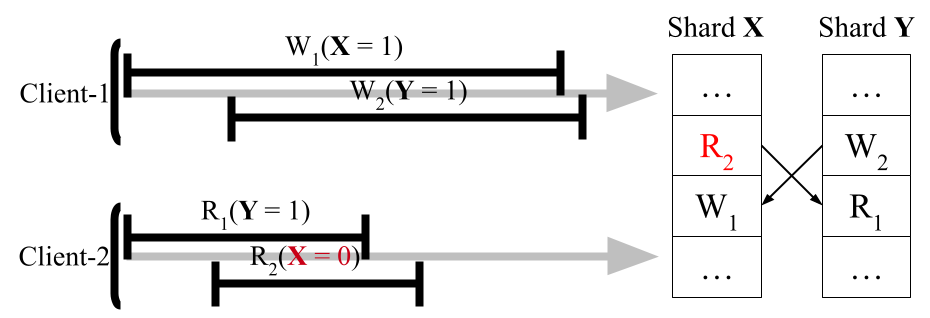
\includegraphics[scale=.45]{figs/somet.png}
    \caption{Example execution where two concurrent clients each submit 2 concurrent requests. Assume keys \textbf{X} and \textbf{Y} are at different shards. It is possible that $R_2$ arrives before $W_1$ at shard \textbf{X}, and $W_2$ arrives before $R_1$ at shard \textbf{Y}. Since clients expect their concurrent requests to take affect in invocation order, if $R_1$ returns 1, then $W_1$ must have taken affect before $R_1$, so $R_2$ should necessarily return a value of 1.}
    \label{fig:concurrentbatches}
\end{figure}

For the single-shard setting, existing protocols come close to providing \MDL{}. A simple mechanism, such as per-client sequence numbers, can provide enough information for a shard leader to support invocation order for multiple requests from a single client. Such a solution does not suffice in the multi-shard setting, however, as shown in figure ~\ref{fig:concurrentbatches}. Linearizability is a local property, thus a single-shard protocol correctly scales to multiple shards. \MDL{}, however, is not a local property due to the possible interleaving of sets of concurrent requests across concurrent clients.
% Jeff: I don't think we want (or need) to make the claim below.
% This requires an \MDL{} protocol to use inter-shard communication in order to guarantee a safe total ordering that reflects issue order.

Sequence numbers are assigned at the client library 
and increase monotonically per shard. For example, a client issuing two requests for the first time to different keys that are on different shards will issue two requests both with sequence number 0. The shard leaders can then easily detect when a client's request
has arrived out of order and can buffer it until the necessary predecessor requests intended for the same shard arrive.
